% Uncomment one of three below
%\RequirePackage[]{optional}
\RequirePackage[notslides]{optional}
%\RequirePackage[slides]{optional}

\opt{slides}{
% Following for presentation mode
\documentclass[10pt]{beamer}
\usepackage{xmpmulti}
%usetheme{Berlin}
}
\opt{notslides}{
% Following for notes mode
\documentclass[a4paper]{article}
\usepackage{beamerarticle}
\usepackage{a4wide}
\usepackage{graphicx}
\usepackage{amsfonts}
\usepackage{fancyhdr}
}

% Following for all modes
%\usepackage{auto-pst-pdf}
%\usepackage{pst-pdf}
\usepackage{psfrag}

\parindent=0ex
\parskip=1ex
\newcommand{\conv}{\ast}
\reversemarginpar

%\title{Signals}
%\author{}
%\date{}

\begin{document}
\pagestyle{fancy}
\fancyhead{}
\renewcommand{\headrulewidth}{0pt}
\fancyfoot[C]{\thesection-\thepage}
%\fancyfoot[R]{fcn2010}

\begin{frame}
  \titlepage
\end{frame}

\setcounter{section}{1}
\section{Signals}

%\mode<article>{{\bf \LARGE Signals} \newline}

We usually use signals to represent quantities that vary with time.  An example of a signal is the size of the sea swell at some location in False Bay:  at any particular time the waves in the bay have an amplitude (size), and this amplitude varies from one moment to the next.  There are buoys in the ocean that measure this quantity, so you can find the information on the internet (the website www.windguru.com reports it for a buoy just off Milnerton).  Surfers and sailors find this information useful because by seeing a recent plot of wave amplitude versus time they know whether they should bother to go out and enjoy the ocean.  Even better, by seeing the current swell size and measuring a whole lot of other signals it is possible to predict what the waves will be like in the short-term future, so you can plan for tomorrow --- this is the basis for weather forecasting.

The swell size can't have two values for an instant in time.  For example, right now it doesn't make sense to say that the size is both 2m and 3m.  This is true for {\em all} quantities that you can measure.  A mathematical function has the same properties:  the function $f(t)$ only provides a {\em single} value for any particular value of the independent variable $t$.  Thus it makes sense to consider a signal to be a {\em function}.

Following the previous example, we could therefore consider the swell size of the waves in a particular location to be a function of time, represented by $s(t)$.  If you know this function and I give you an instant of time $t = t_0$, you can tell me exactly what the value of the function is, $s(t_0)$, and by implication I know the size of the swell.

There are some aspects of signals that can be confusing.  One is this:  as far as the mathematics is concerned a signal exists {\em for all values of time}, so as far as we're concerned the signal $s(t)$ above is known for {\em all} possible values of $t$ --- it makes sense to think of a signal $s(t)$ as an object, rather than as a collection of values.  The fact that we might not have observed the signal for a lot of its existence is irrelevant.  In principle (ignoring the fact that due to continental drift False Bay didn't always exist) there has {\em always} been a specific value of swell size for any instant in time, even though we weren't measuring it.

Another possibly confusing aspect is that, for purposes of the theory, we really need to allow signals to take on {\em complex} values --- for any given $t$ the value of $s(t)$ is therefore a number, but this value may have a real and an imaginary component or a magnitude and a phase.  Admittedly, it's hard to think of a real-world signal that can be complex valued, but as far as the mathematical theory is concerned it is an essential ingredient.  We just have to make sure that our mathematical representation eventually leads to a real-valued signal for any physical variable that it produces.

The upshot is that signals can be represented as functions of time.  It makes sense to represent a signal by a function $s(t)$.  As far as signal processing is concerned, we could work with $s(t)$ as a mathematical entity, and it makes sense to ask questions like "What happens when we put $s(t)$ through a lowpass filter?"  

\subsection{Elementary algebra on signals}

A\marginpar{Lathi sec. 1.3} signal is simply a function, usually of time.  The basic algebra on functions, and therefore of signals, requires an understanding of two operations, addition and multiplication.  

\subsubsection{Addition of signals}

There are two cases that we can think about regarding addition of signals:  we could add a constant value $k$ to a signal $x(t)$, or we could add two signals $x(t)$ and $y(t)$.  In some sense these two cases are equivalent. 

Consider a signal $x(t)$.  A signal is simply a function.  For each value of $t$, the function $x(t)$ returns a value.  If we want to plot a function $x(t)$, we draw an axis representing the independent variable $t$.  Then, for every value of $t$ (the domain of the function), we find the corresponding value of the function $x(t)$ at this instant.  The graph of $x(t)$ then indicates this value for the chosen $t$.  If we repeat this process for all possible values of $t$, the graph traces out a curve that we consider to be the graph of $x(t)$.

The sum of two signals is another signal.  Suppose we know two signals $x(t)$ and $y(t)$.  The sum of these two signals is another signal (or function) that has the form $z(t) = x(t) + y(t)$.  If you want to draw $z(t)$, you choose a value of $t$, say for example $t=2$, and you find the value of $z$ at this point:  $z(2)$.  From the known relation $z(2) = x(2) + y(2)$ you then find the values $x(2)$ and $y(2)$, add them together, and you have $z(2)$.  The graph of $z(t)$ at $t=2$ must pass through this point.  Procedurally, you repeat this operation for {\em every} value of $t$, finding the corresponding values of $z(t)$ from the relation $z(t) = x(t) + y(t)$.  Adding to signals (or functions) in this context is simple (and you know how to do it):  for each value of $t$, add the values of $x(t)$ and $y(t)$, and the result is the value of $z(t)$ at that instant.  In this way you can plot $z(t)$ as a function of time:
\begin{center}
  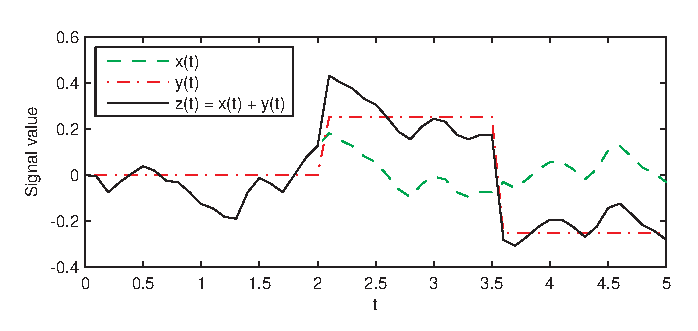
\includegraphics{addsignalsex1}
\end{center}
The signal $z(t)$ is therefore obtained by just adding $x(t)$ to $y(t)$ point by point.

Adding a constant value to a signal is simple.  Suppose $z(t) = x(t) + k$ for some fixed $k$.  For each instant in time $t$, the value of $z(t)$ is just the value of $x(t)$ at the same instant, with the constant $k$ added to it.  The graph of $z(t)$ looks the same as the graph of $x(t)$, but it is shifted in the range direction by a distance $k$.
\begin{center}
  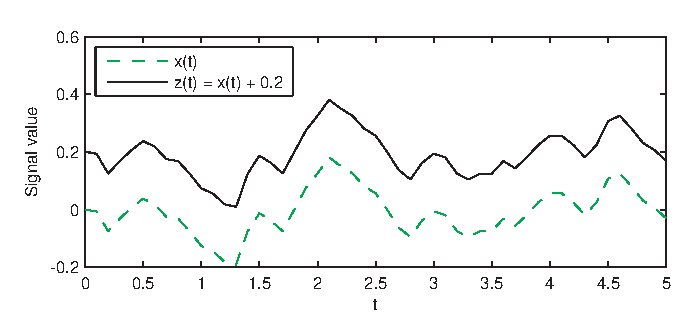
\includegraphics{addsignalsex2}
\end{center}Alternatively, we could think of $z(t) = x(t) + k$ as $z(t) = x(t) + y(t)$ with $y(t) = k$ (a constant signal with value $k$ for all $t$).  

\subsubsection{Multiplication of signals}
In the same way as for addition, two signals can also be multiplied point by point.  If $z(t) = x(t) y(t)$, then the value of $z(t)$ at an instant $t = t_0$ is just the product of the values of $x(t)$ and $y(t)$ at the same instant.  Thus $z(t_0) = x(t_0) y(t_0)$.  This is true for all possible values of $t_0$:
\begin{center}
  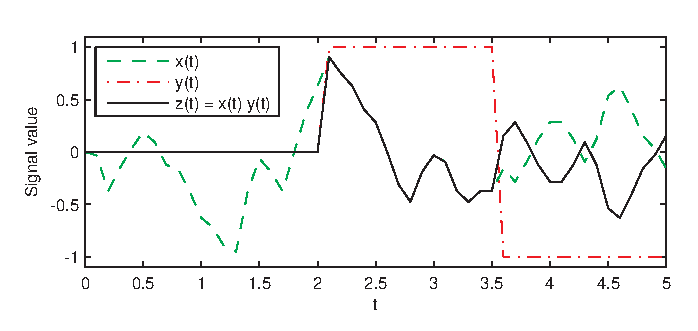
\includegraphics{multsignalsex1}
\end{center}
Multiplication by a constant follows in the obvious way:
\begin{center}
  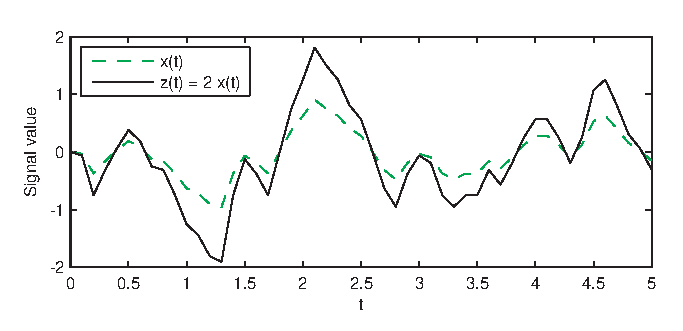
\includegraphics{multsignalsex2}
\end{center}
\marginpar{Lathi prob. 1-5 to 1-7}

\subsection{Basic signals}

To\marginpar{Lathi sec. 1.4} work with signals we need a basic "vocabulary".  There are a number of signals that we will deal with routinely.

\subsubsection{The unit step}

One really simple signal is the unit step, which we denote by $u(t)$.  The definition is simple:
\begin{equation*}
  u(t) = \begin{cases}
    1 \qquad & t \geq 0 \\
    0 \qquad & t<0.
  \end{cases}
\end{equation*}
This is a signal (or function) that has a value of zero for negative values of time, and a value of one for non-negative values of time.  A plot of the unit step follows:
\begin{center}
  \psfrag{t}{\scriptsize $t$}
  \psfrag{u(t)}{\scriptsize $u(t)$}
  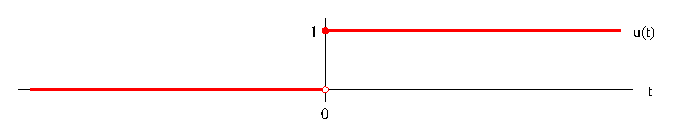
\includegraphics{unitstep}
\end{center}
The interesting point for the unit step happens at $t=0$, where the signal changes value from 0 to 1.  This raises an interesting question, though --- what is negative time?  The answer is that we can put $t=0$ anywhere we like as far as the mathematics is concerned.  I could say that I consider $t=0$ to be the instant when Mandela was inaugurated.  In that case negative time corresponds to pre-1994 and today corresponds to post-1994.  The origin for a signal is important for practical purposes, but for mathematics we can put it wherever is convenient for our purpose.

The unit step signal changes instantaneously from one value (zero) to another (one).  It is therefore useful for representing {\em changes} in signals that occur at specific values of time.  You will see later that it is useful for characterising systems:  if you put a unit step {\em into} a system, then the response of the system to this input is very informative (and is called the {\em step response} of the system).

No real signal can look exactly like a unit step, since it has a discontinuity at $t=0$.  Suppose for example that $u(t)$ represent the value of the current through a particular resistor in a circuit through time.  This would mean that the current would have to change {\em instantaneously} from a value of zero amps to a value of one amp.  This could never occur in reality:  changing a current instantaneously would require infinite energy in practice, and even the universe doesn't contain infinite energy.  Nonetheless, it is valid mathematically and in reality we could make a signal that {\em almost} looks like a unit step --- and it's a particularly useful idealisation.

In signals and systems theory we are able to deal with signals that are undefined at some points.  Strictly speaking, the theory is consistent as long as the signal is defined everywhere except at a countable (but possibly infinite) set of points.  For the unit step $u(t)$ above we don't really want to concern ourselves with what the value is at $t=0$ --- it could be one, as shown, but it could also be zero or any other value.  For purposes of working out what happens when a signal goes through a system, the value at $t=0$ turns out to be irrelevant\footnote{The justification for this lies in what it means for two signals to be equal to one another.  An obvious way to define equality between $f(t)$ and $g(t)$ is to require that $f(t) = g(t)$ for all $t$.  Under this definition the signals $f(t)$ and $g(t)$ have to be defined everywhere.  In signals theory this is {\em not} what we mean by equality.  Rather, we consider the two signals to be equal if $\int_{-\infty}^{\infty} (f(t) - g(t))^2 dt = 0$:  there must be zero energy in the {\em difference} between $f(t)$ and $g(t)$.  This is a much less strict definition of equality, since the two signals can be different from one another as long as the difference has zero (squared) area.  This is also a more physically meaningful measure of similarity:  any physical device that measures a signal {\em has} to have some energy transferred to it, so if two signals are equivalent in terms of energy then there is no practical way of telling them apart.}.  We can express our ambivalence formally by just leaving $u(t)$ undefined at $t=0$, and representing the unit step as below:
\begin{center}
  \psfrag{t}{\scriptsize $t$}
  \psfrag{u(t)}{\scriptsize $u(t)$}
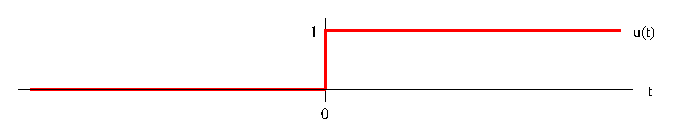
\includegraphics{unitstep2}
\end{center}
As drawn, $u(t)$ is not a function --- it takes on all possible values between zero and one at $t=0$, while a function must be single valued.  The graph above would be unacceptable in formal mathematics, but for our applications it conveys the required information.
\marginpar{Lathi prob. 1-8 to 1-9}

\subsubsection{Sinusoidal signals}

An general canonical sinusoidal signal takes the form
\begin{equation*}
  s(t) = A \cos(\omega t + \phi),
\end{equation*}
where $A$ is the amplitude (half of the peak-to-peak variation), $\omega$ is the frequency (in radians/second), and $\phi$ is the phase, which basically corresponds to a specification of the position of the sinusoid along the time axis.  Why is this called a sinusoid while there's a "$\cos$" in the expression?  Well, since $\sin(x) = \cos(x-\pi/2)$, the only difference between a $\sin$ and a $\cos$ is a phase shift, which can be accommodated by an appropriate value of $\phi$.  Thus when we talk about sinusoids we mean the class of signals that varies in a way that looks harmonic, without paying too much attention to the exact form of the function specified.  

A signal $x(t)$ is periodic with a period of $T$ if $x(t) = x(t+T)$ for all $t$.  For the sinusoidal signal above to be periodic we therefore require that
\begin{equation*}
  A \cos(\omega t + \phi) = A \cos(\omega (t+T) + \phi) = A \cos(\omega t + \omega T + \phi)
\end{equation*}
for all $t$, which is true as long as $\omega T = 2 \pi k$ for some integer $k$.  The smallest value of $T$ for which this is true is for $k=1$, so the {\em fundamental period} of the signal is $T = \frac{2 \pi}{\omega}$.  

The phase $\phi$ of a sinusoid determines the position of the signal along the time axis.  Suppose for now that $\phi = 0$.  The signal $s(t)$ above then corresponds to a sinusoid that takes on its peak value of $A$ at $t=0$.  However, for nonzero phase we can write the signal as $x(t) = A \cos(\omega (t + \frac{\phi}{\omega}))$, which is just the signal $A \cos(\omega t)$ shifted to the left by $\frac{\phi}{\omega} = \frac{\phi}{2 \pi} T$.  It is evident then that a specified phase shift shifts the signal in time by an amount that is proportional to $T$, the wavelength of the sinusoid.  The phase therefore determines the shift of the signal measured in units of the wavelength, rather than in units of time.
\subsubsection{The complex exponential}

The complex exponential is the most important signal in the theory of signals and systems.  A complex exponential of frequency $\omega$ radians per second can be expressed as
\begin{equation*}
  s(t) = e^{j \omega t},
\end{equation*}
where $j = \sqrt{-1}$.  This is an example of a complex-valued signal (or function), since by Euler's formula we can write it in the rectangular form
\begin{equation*}
  s(t) = \cos(\omega t) + j \sin(\omega t).
\end{equation*}
Thus it has a real component of $\cos(\omega t)$ and an imaginary component of $\sin(\omega t)$, both of which are sinusoidal.  Alternatively, it has a constant magnitude of 1 and a phase of $\omega t$.

The complex exponential is probably the only signal that you'll ever see that contains both an $t$ variable and a $\omega$ variable in its expression.  This isn't a coincidence:  it's the signal that links the two domains of time and frequency.  When we talk about the component of a signal at frequency $\omega$, we're really referring to the part of the signal that "looks" like $e^{j \omega t}$.

Because a complex exponential signal takes on complex values we can only really visualise it using two plots.  Below are plots of the real part and the imaginary part of a complex exponential signal with frequency $\omega = 2 \pi$:
\begin{center}
  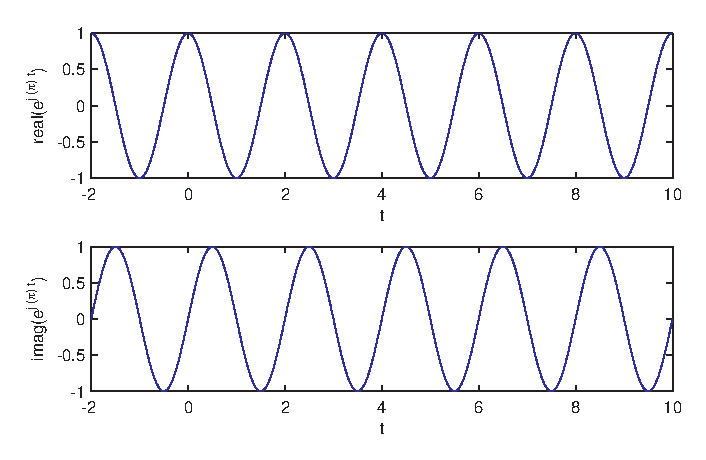
\includegraphics{complexexpplot} 
\end{center}
Alternatively, the same complex exponential could be represented in magnitude and phase form, leading to the two plots below:
\begin{center}
  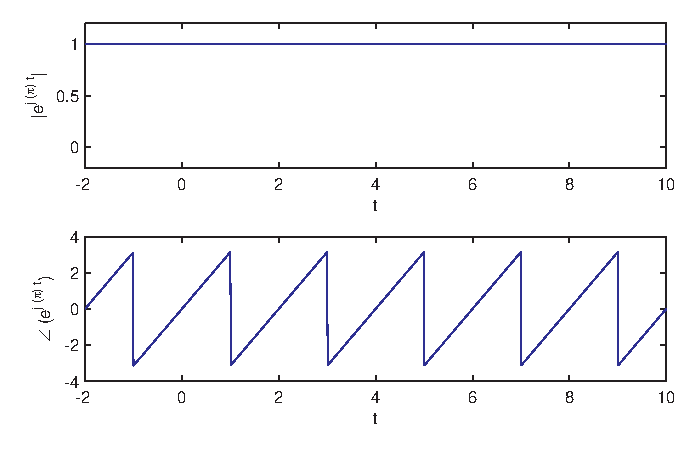
\includegraphics{complexexpplot2} 
\end{center}
Note that the phase is $\omega t$, which is a straight line, but since we can't tell the difference between a phase of zero and a phase of $2 \pi$ we normally plot it in the range $-\pi$ to $-\pi$ (which leads to the triangular phase plot above).  An unconventional but otherwise informative way of visualising it is shown below:
\begin{center}
  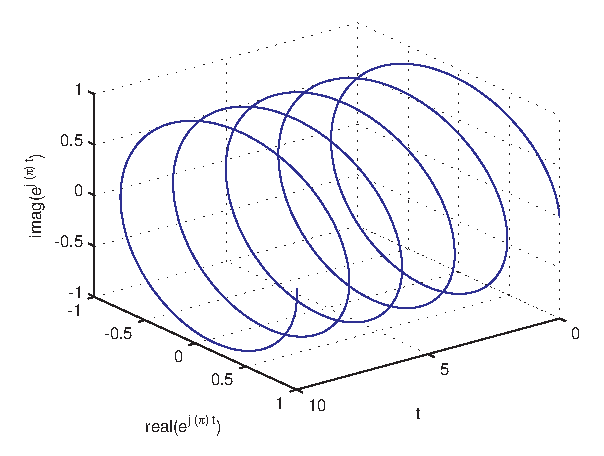
\includegraphics{complexexpplot3} 
\end{center}

The complex exponential signal of frequency $\omega$ is easily shown to be periodic.  Assuming a period $T$, the required condition is that $e^{j \omega t} = e^{j \omega (t + T)} = e^{j \omega t} e^{j \omega T}$.  This holds as long as $e^{j \omega T} = 1$, so we must have $\omega T = 2 \pi k$ for some integer $k$.  As for the case of the sinusoid, the fundamental period is therefore $T = \frac{2 \pi}{\omega}$.

Most of Fourier analysis involves forming weighted sums (or linear combinations) of complex exponentials.  To this end it's really useful to have a clear picture of what it means to multiply a complex exponential by a constant, generally complex valued.  Let $x(t) = e^{j \omega t}$ be a complex exponential and consider the signal $y(t) = z x(t)$, where $z$ is complex and can therefore be written as $z = \rho e^{j \phi}$.  Then
\begin{equation*}
  y(t) = z x(t) = \rho e^{j \phi} e^{j \omega t} = \rho e^{j (\omega t + \phi)}
  = \rho e^{j \omega (t + \frac{\phi}{\omega})} = \rho x(t + \frac{\phi}{\omega}).
\end{equation*}
The signal $y(t)$ is therefore {\em still a complex exponential at frequency $\omega$}.  Its amplitude (or magnitude) has been scaled by $\rho = |z|$ and it has been shifted in time by $-\frac{\phi}{\omega}$, but it aside from that it's the same signal.  Thus multiplying a complex exponential by a complex value leaves the frequency constant, just changing its magnitude and its phase.

Finally, note that there's nothing in the theory that requires $\omega \geq 0$.  Negative frequencies exist and make sense:  the just correspond to a complex exponential with a negative in the exponent.  For example, the complex exponential signal $e^{-j \pi t}$ has a frequency of $\omega = - \pi$, and it's not the same signal as $e^{j \pi t}$ of frequency $\omega = \pi$.  

{\em Earlier\marginpar{\bf Exercise:} in this section you were shown the signal $e^{j \pi t}$ in real and imaginary form, and in magnitude and phase form.   Draw (or use a computer to draw) equivalent plots for the signal $e^{-j \pi t}$, and convince yourself that these two signals are different (but equally legitimate).}

\subsubsection{The Dirac delta}

The Dirac delta function is not a function in the usual sense (actually it's an instance of something called a distribution function, which is like a generalised function).  However, it is also one of the most important functions in signals and systems theory.

The Dirac delta $\delta(t)$ can be defined in terms of two properties:
\begin{gather*}
  \delta(t) = 0 \quad \text{for} \quad t \neq 0 \\
  \int_{-\epsilon}^{\epsilon} \delta(t) dt = 1 \quad \text{for all} \quad \epsilon > 0.
\end{gather*}
The first condition says that the Dirac delta is zero almost everywhere along the time axis.  The only instant in time where it is nonzero is at the origin.  Note that the value $\delta(0)$ is not defined.  The second condition says that if we integrate the delta function over any interval that includes the origin, then we get a value of 1.  In other words, the area underneath the delta function over any interval that includes the origin is unity.  

It's a strange definition:  we couldn't draw $\delta(t)$ since it's not really a function.  There is however a way of visualising it as a limiting process.  To formulate it in this manner, we first need to define another signal, the unit pulse of total width $T$:
\begin{center}
  \psfrag{t}{\scriptsize $t$}
  \psfrag{T/2}{\scriptsize $\frac{T}{2}$}
  \psfrag{-T/2}{\scriptsize $-\frac{T}{2}$}
  \psfrag{p_T(t)}{\scriptsize $p_T(t)$}
  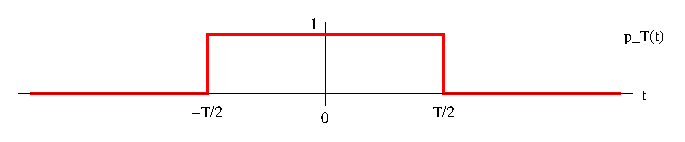
\includegraphics{unitpulse}
\end{center}
It is zero everywhere, except in the range $[-T/2, T/2]$ where it has a value of one.  As for the case of the unit step, we've drawn this signal with vertical lines at $-T/2$ and $T/2$, expressing the fact that we are indifferent to its value at these points.  

{\em Convince\marginpar{\bf Exercise:} yourself that $p_T(t) = u(t + T/2) - u(t - T/2)$, where $u(t)$ is the unit step defined earlier.}

Now consider the signal $T p_{\frac{1}{T}}(t)$, shown below:
\begin{center}
  \psfrag{t}{\scriptsize $t$}
  \psfrag{T}{\scriptsize $T$}
  \psfrag{1/2T}{\scriptsize $\frac{1}{2T}$}
  \psfrag{-1/2T}{\scriptsize $-\frac{1}{2T}$}
  \psfrag{Tp_1/T(t)}{\scriptsize $T p_{\frac{1}{T}}(t)$}
  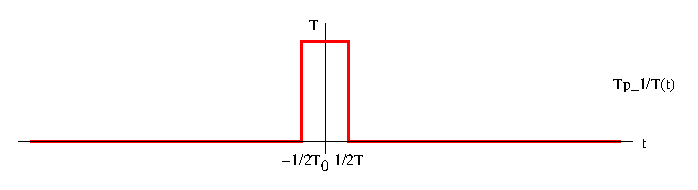
\includegraphics{diracrect}
\end{center}
It has a height of $T$ and a total width of $1/T$.  It shares a lot of the properties of the Dirac delta as defined.  It is zero everywhere, except on the interval $[-\frac{1}{2T}, \frac{1}{2T}]$.  Also, since the signal is a rectangle of height $T$ and width $1/T$ it has a total area of one, so as long as we choose $\epsilon \geq T/2$ we find that $\int_{-\epsilon}^{\epsilon} T p_{\frac{1}{T}}(t) dt = 1$.  To make this signal really behave like a delta function, we need to take the limit as $T \to \infty$.  The pulse then becomes infinitely narrow and infinitely high, but still has an area of one.  We could therefore reasonably define the delta function as
\begin{equation*}
  \delta(t) = \lim_{T \to \infty} T p_{\frac{1}{T}}(t).
\end{equation*}
The interval $[-\frac{1}{2T}, \frac{1}{2T}]$ over which the pulse above is nonzero becomes infinitely small as $T \to \infty$, so the first condition in the Dirac delta definition is met.  Also, if you pick any value of $\epsilon > 0$ it defines the interval $[-\epsilon, \epsilon]$.  For $T \to \infty$ the entire pulse, which always has unit area, is contained in this interval.  Therefore
\begin{equation*}
  \int_{-\epsilon}^{\epsilon} \lim_{T \to \infty} T p_{\frac{1}{T}}(t) = 1.
\end{equation*}
The second condition in the definition is therefore also met.

It's an advanced topic, but the reason that distribution functions work is because in principle we can do all our mathematics with the signal $T p_{\frac{1}{T}}(t)$ instead of with $\delta(t)$.  All the results will then depend on $T$.  However, {\em after} we're finished we can take the limit as $T \to \infty$, so the $T$ disappears.  The theory of distribution functions says that for most purposes it doesn't matter when we take this limit:  {\em before} or {\em after} is just as good.  There are whole textbooks written on the theory, but since other people have determined that it works we simply use it as a tool.

Since a Dirac delta is not really a function, we can't draw it.  The convention is therefore adopted that we represent $\delta(t)$ as shown below:
\begin{center}
  \psfrag{t}{\scriptsize $t$}
  \psfrag{delta(t)}{\scriptsize $\delta(t)$}
  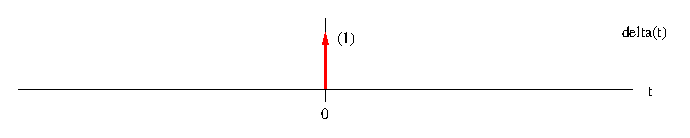
\includegraphics{deltafunction}
\end{center}
The notion is suggestive:  the function as shown is clearly zero everywhere except at the origin, as required.  At the origin, however, we don't indicate a value, but rather use an upward arrow.  The $(1)$ next to the arrow indicates that it has an effective area of 1.

It also makes sense to think about a delta function multiplied by a constant value.  For example, the signal $5 \delta(t)$ can be thought of as the function $5 T p_{\frac{1}{T}}(t)$, in the limit as $T \to \infty$.  Since the area under $5 T p_{\frac{1}{T}}(t)$ is always exactly 5, we can see that
\begin{equation*}
  \int_{-\epsilon}^{\epsilon} 5 T p_{\frac{1}{T}}(t) dt = 5
\end{equation*}
as long as $\epsilon \geq \frac{1}{T}$.  Taking the limit as $T \to \infty$ of the above we see that
\begin{equation*}
  \int_{-\epsilon}^{\epsilon} 5 \delta(t) dt = 5
\end{equation*}
for all $\epsilon > 0$, so the total area under $5 \delta(t)$ is five.  Using the same representation as before we would draw the signal as follows:
\begin{center}
  \psfrag{t}{\scriptsize $t$}
  \psfrag{5delta(t)}{\scriptsize $5 \delta(t)$}
  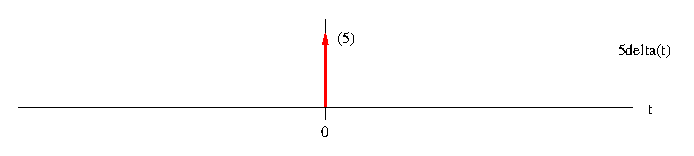
\includegraphics{deltafunction5}
\end{center}
The $(5)$ next to the arrow now indicates that the delta has a {\em size} or {\em weight} of 5, in the sense that the total area underneath the arrow is 5 units.  Alternatively, the arrow as indicated has $5$ units of area associated with it.

From the definition of the Dirac delta we can determine that it is an even function.  Let $\delta_{-}(t)$ be the time-reversed delta function, so $\delta_{-}(t) = \delta(-t)$.  Since $\delta(t) = 0$ for $t \neq 0$ it must be true that $\delta_{-}(t) = $ for $t \neq 0$.  Also,
\begin{equation*}
  \int_{-\epsilon}^{\epsilon} \delta_{-}(t) dt = \int_{-\epsilon}^{\epsilon} \delta(-t) dt = \int_{-\epsilon}^{\epsilon} \delta(\tau) d\tau = 0
\end{equation*}
for all $\epsilon > 0$, where the variable substitution $\tau = -t$ has been used.  Thus $\delta_{-}(t)$ is a function that satisfies exactly the same properties as were used to define $\delta(t)$, so it must be true that $\delta(t) = \delta_{-}(t) = \delta(-t)$ and $\delta(t)$ is even.  Alternatively, since we constructed the delta function in a limit process from a rectangular pulse, which is even, it seems evident that $\delta(t)$ must itself be even.

\subsection{Using the theory}

\subsubsection{Sifting property of the delta function}

Think about any signal $x(t)$, and consider an instant $t_0$ in time.  The sifting property of the delta function states that
\begin{equation*}
  \int_{-\infty}^{\infty} x(t) \delta(t - t_0) dt = x(t_0).
\end{equation*}
Whenever you are faced with a statement that you don't understand, it usually helps to draw something that you {\em do} understand.  In this case, we should think about the quantity inside the integral, $x(t) \delta(t - t_0)$.  It's clearly a function of time $t$, and $t_0$ is a fixed constant number.  It's also the {\em product} of two signals, namely $x(t)$ and $\delta(t - t_0)$.  The signal $\delta(t - t_0)$ is a delta function, but it has been shifted in time so that it occurs at time $t = t_0$.  The two signals and their product are shown below:
\begin{center}
  \psfrag{t}{\scriptsize $t$}
  \psfrag{t_0}{\scriptsize $t_0$}
  \psfrag{x(t)}{\scriptsize $x(t)$}
  \psfrag{x(t_0)}{\scriptsize $x(t_0)$}
  \psfrag{(x(t_0))}{\scriptsize $(x(t_0))$}
  \psfrag{d(t-t_0)}{\scriptsize $\delta(t-t_0)$}
  \psfrag{x(t)d(t-t_0)}{\scriptsize $x(t) \delta(t-t_0)$}
  \psfrag{f(t)=x(t_0)}{\scriptsize $f(t)=x(t_0)$}
  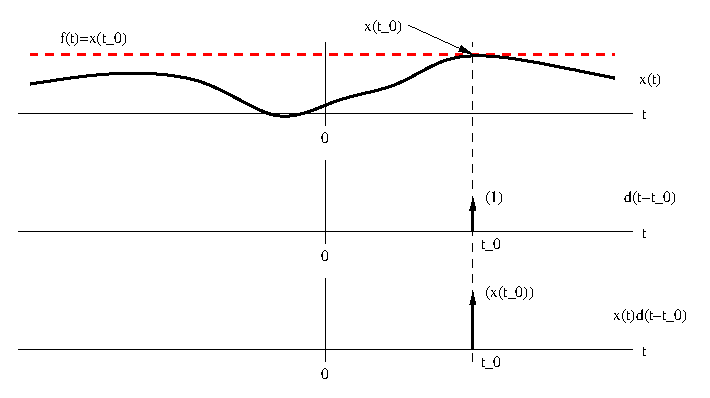
\includegraphics{siftingproperty}
\end{center}
The signal $x(t) \delta(t - t_0)$ (shown at the bottom) is a delta function at $t = t_0$, but it now has an area (or size) of $x(t_0)$ since $\delta(t-t_0)$ has been multiplied by the value of $x(t)$ at the same time instant.  The sifting property is claiming that the total area underneath this bottom function is $x(t_0)$, which is obviously true --- the plot only contains a delta function of size $x(t_0)$, which almost by definition has an area of $x(t_0)$.

The sifting property lets you do some interesting algebra.  Instead of the signal $x(t)$ above, suppose the signal was the constant signal $f(t)$ shown as a dotted red line.  The product $f(t) \delta(t - t_0)$ would look exactly the same as the bottom plot:  the delta function only "samples" the value of the top signal at $t=t_0$, and both $x(t)$ and $f(t)$ have exactly the same value at this point.  
Thus
\begin{equation*}
  x(t) \delta(t-t_0) = f(t) \delta(t-t_0) = x(t_0) \delta(t - t_0),
\end{equation*}
since when you plot these they look exactly the same.  

{\em Suppose\marginpar{\bf Exercise:} $x(t) = sin(\pi t)$ and $t_0 = 1/4$.  Plot $x(t) \delta(t-t_0)$ and $x(t_0) \delta(t - t_0)$.  These two signals should look {\em exactly} the same.  Convince yourself that this would be true for {\em any} signal $x(t)$ and {\em any} value $t_0$.}

Since the integrands are identical, we must have
\begin{equation*}
  \int_{-\infty}^{\infty} x(t) \delta(t-t_0) dt = \int_{-\infty}^{\infty} x(t_0) \delta(t - t_0) dt.
\end{equation*}
However, $x(t_0)$ is constant (since we chose $t_0$).  We can therefore take it out of the integral, and the sifting property follows:
\begin{equation*}
  \int_{-\infty}^{\infty} x(t) \delta(t-t_0) dt = \int_{-\infty}^{\infty} x(t_0) \delta(t - t_0) dt
  = x(t_0) \int_{-\infty}^{\infty} \delta(t - t_0) dt = x(t_0).
\end{equation*}
Note that this last integral vanishes because a shifted delta function has unit area.

The previous statement leads to the following procedure.  Since the integrand $x(t) \delta(t-t_0)$ is only nonzero when $t = t_0$, {\em it doesn't matter what the value $x(t)$ is except at $t=t_0$}.  Inside the integral we can therefore replace all instances of $t$ (except the one associated with the delta function) with the value $t_0$.  This change doesn't change the thing that is being integrated.  Thus
\begin{equation*}
  \int_{-\infty}^{\infty} x(t) \delta(t-t_0) dt = \int_{-\infty}^{\infty} x(t_0) \delta(t-t_0) dt.
\end{equation*}

Finally, the sifting property also lets us write any signal $x(t)$ in an interesting and useful form:
\begin{equation*}
  x(t) = \int_{-\infty}^{\infty} x(\tau) \delta(t - \tau) d\tau.
\end{equation*}
Suppose we choose a value of $t$ and want to calculate $x(t)$.  In the above expression $t$ is then a fixed value, and $\tau$ is the integration variable.  When considered as a function of $\tau$, the integrand is only nonzero when $\tau = t$, so inside the integral we can replace $x(\tau)$ with $x(t)$ without changing the quantity being integrated.  Thus
\marginpar{Lathi prob. 1-11 to 1-12}
\begin{equation*}
  \int_{-\infty}^{\infty} x(\tau) \delta(t - \tau) d\tau = \int_{-\infty}^{\infty} x(t) \delta(t - \tau) d\tau
  = x(t) \int_{-\infty}^{\infty} \delta(t - \tau) d\tau = x(t).
\end{equation*}

{\em You\marginpar{\bf Exercise:} really need to be clear about what it means to be integrating over a variable.  In the expression $\int_{-\infty}^{\infty} x(\tau) \delta(t - \tau) d\tau$, the variable $\tau$ is the integration variable, and in this expression $t$ is a constant.  To evaluate the integral you should therefore think about a fixed value of $t$, and plot $x(\tau)$, $\delta(t - \tau)$, and $x(\tau) \delta(t - \tau)$ as a function of $\tau$.  Repeat the previous example in this context, and convince yourself that the expression (or decomposition) of $x(t)$ above is correct.}

\subsubsection{The generalised derivative}

The standard formulation of calculus defines differentiation in terms of gradients in a limiting process.  If a function $f'(t)$ is the derivative of the function $f(t)$, then at any time instant $t=t_0$ we must have
\begin{equation*}
  f'(t_0) = \lim_{h \to 0} \frac{f(t_0+h) - f(t_0)}{h}.
\end{equation*}
To use this expression to calculate the derivative at $t_0$, the value $f(t_0)$ must be defined.  Also, for the limit to be meaningfully defined it must not matter whether $h \to 0$ from the positive side or from the negative side:  the same value must be obtained in the limit for both cases.  

Consider the signals below:
\begin{center}
  \psfrag{t}{\scriptsize $t$}
  \psfrag{f(t)}{\scriptsize $f(t)$}
  \psfrag{g(t)}{\scriptsize $g(t)$}
  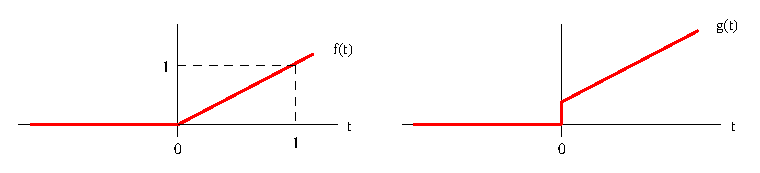
\includegraphics{genderivex1}
\end{center}
The signal $f(t)$ exhibits the second problem just outlined.  While it is defined everywhere (including at $t=0$), the slope depends on which side of the origin we are on:  for negative $t$ it is zero, while for positive $t$ it is one.  Thus the slope as we approach the origin from the left is 0, while it is 1 if we approach from the right.  Since no meaningful value can be determined for $f'(0)$, the derivative doesn't exist at the origin.

The signal $g(t)$ exhibits both problems.  At the origin its value is not defined, as indicated by the vertical line at this point on the graph.  Since $g(0)$ is not defined, we can't even begin to use the formula to find the derivative.  The slope when approaching $t=0$ from the left and from the right is also different, so the second problem also still persists.

In order to meaningfully define a derivative for the signals above we therefore need to proceed in a different manner.  A solution is to think of the inverse process of differentiation, namely {\em indefinite integration}.  If $y(t) = \frac{d}{dt} x(t)$, then elementary calculus lets us express $x(t)$ in terms of $y(t)$:
\begin{equation*}
  x(t) = \int_{-\infty}^t y(\tau) d\tau.
\end{equation*}
Note the appearance of the $t$ in the integration limits, and the use of the dummy variable $\tau$.  Admittedly there could be an undetermined integration constant added to the right-hand side, but it is not important for our purposes:  essentially we're assuming that $x(-\infty) = 0$, which is called the {\em initial rest} condition.

\begin{center}
\fbox{
\begin{minipage}{0.9\textwidth}
Since differentiation and indefinite integration are inverse operations, we proceed to define differentiation in terms of integration:  the generalised derivative of $x(t)$ is the function $x'(t)$ which, when it is integrated in the indefinite sense, yields $x(t)$.  
\end{minipage}
}
\end{center}

Consider for example the indefinite integral of the Dirac delta function:  $x(t) = \int_{-\infty}^t \delta(\tau) d\tau$.  The value of $x(t)$ at $t=-5$ is $x(-5) = \int_{-\infty}^{-5} \delta(\tau) d\tau$, which can be evaluated and returns a number.  To find this number it is easiest to draw the function being integrated:
\begin{center}
  \psfrag{tau}{\scriptsize $\tau$}
  \psfrag{delta(tau)}{\scriptsize $\delta(\tau)$}
  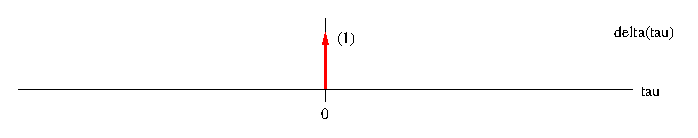
\includegraphics{deltafunctiontau}
\end{center}
The value of $x(-5)$ is the area underneath this function over the interval $(-\infty, -5]$, and since the function is always zero over this range we clearly have $x(-5) = 0$.  On the other hand, $x(5) = \int_{-\infty}^{5} \delta(\tau) d\tau$ is the area under the delta function drawn over the range $(-\infty, 5]$.  The signal is not zero over this range --- it includes a delta function of weight 1, which has exactly one unit of area.  Thus $x(5) = 1$.  

For any value of $t$, the signal $x(t)$ has a value equal to the area underneath $\delta(\tau)$ over the interval $(\infty, t]$.  For $t<0$ we are not integrating over the delta function at the origin, so $x(t) = 0$.  For $t>0$ the integration {\em always} includes the delta function at the origin, so $x(t) = 1$.  We don't know what the value of $x(t)$ for $t=0$, so we leave it undefined.  In any case, we can draw the indefinite integral $x(t)$ as follows:
\begin{center}
  \psfrag{t}{\scriptsize $t$}
  \psfrag{x(t)}{\scriptsize $x(t)$}
  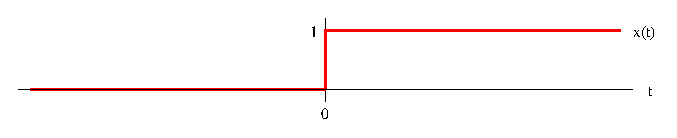
\includegraphics{unitstep3}
\end{center}
Thus we see that the indefinite integral of the delta function is the unit step.  According to the definition of the generalised derivative, the derivative of the unit step is therefore the delta function.

Now consider again the function $g(t)$ shown earlier in this section.  It isn't defined at $t=0$ and certainly doesn't have a derivative at this point.  Nonetheless, in the same way we can define the generalised derivative $g'(t)$ to be the function which, when integrated in the indefinite sense, yields $g(t)$.  Specifically, we are looking for a signal $g'(t)$ such that
\begin{equation*}
  g(t) = \int_{-\infty}^t g'(\tau) d\tau.
\end{equation*}
Once you see the answer you'll quickly work out how to construct generalised derivatives.  

Consider the signal $x(t)$ shown below, also expressed as a function of $\tau$ in the form of $x(\tau)$:
\begin{center}
  \psfrag{t}{\scriptsize $t$}
  \psfrag{x(t)}{\scriptsize $x(t)$}
  \psfrag{tau}{\scriptsize $\tau$}
  \psfrag{x(tau)}{\scriptsize $x(\tau)$}
  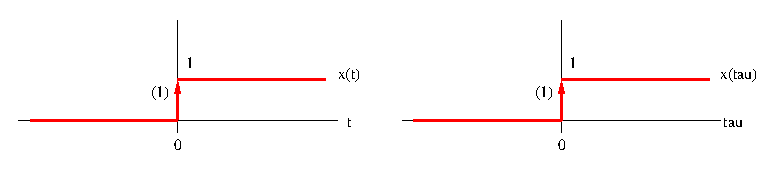
\includegraphics{genderivex2}
\end{center}
We want to calculate the indefinite integral $y(t) = \int_{-\infty}^t x(\tau) d\tau$.  For $t<0$, the area underneath this curve over the interval $(-\infty,t]$ is zero, so $y(t)) = 0$ in this range.  For $t$ an infinitesimal distance to the right of the origin, indicated $t = 0^+$, the integral is over the range $(-\infty,0^+]$.  This includes the delta function at the origin, which has area 1, so $y(0^+) = 1$.  For $t>0$, the integral is over the range $(-\infty,t]$, which includes the impulse at the origin as well as $t$ units of area contributed by the usual part of the integral.  Thus $y(t) = 1 + t$ over this range.  The function $y(t)$ is thus identical to $g(t)$.  

Since the integral of the function $x(t)$ above is $g(t)$, it follows that $x(t)$ is the generalised derivative of $g(t)$.  Thus the pair below form an integral-derivative pair:
\begin{center}
  \psfrag{t}{\scriptsize $t$}
  \psfrag{g(t)}{\scriptsize $g(t)$}
  \psfrag{g'(t)}{\scriptsize $g'(t)$}
  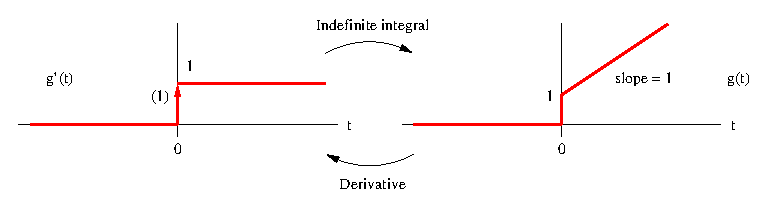
\includegraphics{genderivex3}
\end{center}
Evidently the derivative of $g(t)$ can be written in the analytical form $g'(t) = u(t) + \delta(t)$.  The first term, $u(t)$ is the ordinary derivative (gradient of the function) ignoring any discontinuities.  The second term, $\delta(t)$ is an impulse of size $1$ at the origin, and contributes to the discontinuity of size 1 at the origin in $g(t)$.

Some thought should lead to the following conclusion.  The generalised derivative consists of two parts:  one is the ordinary derivative (or slope) of the signal, ignoring any discontinuities.  In the example above this is the part $u(t)$.  However, there is an additional component comprised of delta functions, which accounts for any discontinuities in the signal being differentiated.  For the case of $g(t)$, if we "walk" along the signal from left to right there is a discontinuity of size 1 at $t=0$.  This is accounted for in the derivative by a Dirac delta of size 1 at $t=0$, or in other words by including a term $1 \delta(t)$.  In general we need one impulse located at each point of discontinuity, and its weight will be the size of the discontinuity.  Note that if the function takes a sudden discontinuous step downwards at a point, then the generalised derivative will contain a negative impulse of the appropriate size at that point.
\marginpar{Lathi prob. 1-13 to 1-14}

\end{document}

